% ------------------------------------------------------------------------------
% LaTeX Template: Titlepage
% This is a title page template which be used for both articles and reports.
%
% Copyright: http://www.howtotex.com/
% Date: April 2011
% ------------------------------------------------------------------------------

% -------------------------------------------------------------------------------
% Preamble
% -------------------------------------------------------------------------------
\documentclass[paper=letterpaper]{article}		

\usepackage[letterpaper,pdftex]{geometry}										% A4paper margins
\setlength{\oddsidemargin}{5mm}												% Remove 'twosided' indentation
\setlength{\evensidemargin}{5mm}
\usepackage[small,compact]{titlesec}
%\usepackage[backend=biber]{biblatex}
\usepackage[spanish]{babel}
\usepackage{epsfig}
\usepackage{array}
\usepackage{xfrac}
\usepackage{amsthm}
\usepackage{amsmath}
\usepackage{todonotes}
\usepackage{centernot}
\usepackage{multicol}
\usepackage{blindtext}
\usepackage{wasysym}
\usepackage{siunitx}
%\usepackage[letterpaper]{geometry}
%\usepackage{multicol}
\usepackage{color}

\usepackage[protrusion=true,expansion=true]{microtype}	
\usepackage{amsmath,amsfonts,amsthm,amssymb}
\usepackage{multicol}
\usepackage{mathtools}
\usepackage{graphicx}
\usepackage{multirow}
\usepackage[small,it]{caption}
%\usepackage{titling}
\usepackage{graphicx}
\bibliographystyle{plain}
%\bibliographystyle{babplain}
\usepackage{filecontents}
\usepackage{titlesec}
\usepackage[section]{placeins}
\usepackage[hidelinks]{hyperref}
\usepackage{fancyhdr}
\usepackage{cancel}
\usepackage{abstract}
\usepackage{tikz}
\usetikzlibrary{trees}



% ------------------------------------------------------------------------------
% Definitions (do not change this)
% ------------------------------------------------------------------------------

\renewcommand{\thesubsection}{\thesection.\alph{subsection}}

\captionsetup[table]{name=Tabla}


\pagestyle{fancy}
\usepackage[utf8]{inputenc}
\fancyhf{}
\fancyhead[c]{\textbf{\textit{Tarea 1} : Edgar A. Margffoy - 201412566 (\S 9) / Sergio Galindo - 201413974 (\S 1)}}
\fancyfoot[c]{\thepage}
\def\Section {\S}

\newcommand\tstrut{\rule{0pt}{2.4ex}}
\newcommand\bstrut{\rule[-1.0ex]{0pt}{0pt}}

\newcommand{\squishlist}{
 \begin{list}{$\bullet$}
  { \setlength{\itemsep}{0pt}
     \setlength{\parsep}{3pt}
     \setlength{\topsep}{3pt}
     \setlength{\partopsep}{0pt}
     \setlength{\leftmargin}{1.5em}
     \setlength{\labelwidth}{1em}
     \setlength{\labelsep}{0.5em} } }


\newcommand{\squishlisttwo}{
 \begin{list}{$\bullet$}
  { \setlength{\itemsep}{0pt}
    \setlength{\parsep}{0pt}
    \setlength{\topsep}{0pt}
    \setlength{\partopsep}{0pt}
    \setlength{\leftmargin}{2em}
    \setlength{\labelwidth}{1.5em}
    \setlength{\labelsep}{0.5em} } }

\newcommand{\squishend}{
  \end{list}  }
\footskip = 50pt
\setlength{\skip\footins}{10pt}

\newcounter{proofc}
\renewcommand\theproofc{(\arabic{proofc})}
\DeclareRobustCommand\stepproofc{\refstepcounter{proofc}\theproofc}
\newenvironment{twoproof}{\tabular{@{\stepproofc}c|l}}{\endtabular}


\newcommand{\HRule}[1]{\rule{\linewidth}{#1}} 	% Horizontal rule

\makeatletter							% Title
\def\printtitle{%						
    {\centering \@title\par}}
\makeatother									

\makeatletter							% Author
\def\printauthor{%					
    {\centering \large \@author}}				
\makeatother							

% ------------------------------------------------------------------------------
% Metadata (Change this)
% ------------------------------------------------------------------------------
\title{	\normalsize \textsc{Universidad de los Andes} \\ 	% Subtitle of the document
         \normalsize            \textsc{Departamento de Ingenier\'{i}a Industrial} \\
         \normalsize            \textsc{Probabilidad y Estad\'{i}stica I}
		 	\\[2.0cm]													% 2cm spacing
			\HRule{0.5pt} \\
			\bigskip										% Upper rule
			\LARGE \textbf{\uppercase{Tarea 1}}	% Title
			\bigskip
			\HRule{0.5pt} \\ [0.5cm]								% Lower rule + 0.5cm spacing
			\normalsize \today									% Todays date
		}

\author{
\begin{multicols}{2}
		Edgar Andr\'{e}s Margffoy Tuay\\	
		201412566\\	
		Secci\'{o}n 9\\
        \texttt{ea.margffoy10@uniandes.edu.co} \\
        \columnbreak
        Sergio Alberto Galindo Le\'{o}n\\
        201413974\\
        Secci\'{o}n 1\\
        \texttt{sa.galindo10@uniandes.edu.co} \\
\end{multicols}
}


\begin{document}
% ------------------------------------------------------------------------------
% Maketitle
% ------------------------------------------------------------------------------
			% Remove page numbering on this page
\def\maketitle
{
\thispagestyle{empty}	
\printtitle									% Print the title data as defined above
  	\vfill
\printauthor}
\maketitle								% Print the author data as defined above
% ------------------------------------------------------------------------------
% Begin document
% ------------------------------------------------------------------------------
\newpage
\begin{table}[!htbp]
\centering
\begin{tabular}{|>{\centering}p{4cm}|>{\centering}p{1cm}|r|}
\hline
\multicolumn{2}{ |c| }{\textbf{Numeral}} &  \textbf{Puntaje} \\
\hline
\multirow{12}{*}{\textbf{1}} & a) & /1 \\ \cline{2-3}
& b) & /3 \\ \cline{2-3}
& c) & /1 \\ \cline{2-3}
& d) & /2 \\ \cline{2-3}
& e) & /2 \\ \cline{2-3}
& f) & /2 \\ \cline{2-3}
& g) & /2 \\ \cline{2-3}
& h) & /2 \\ \cline{2-3}
& i) & /2 \\ \cline{2-3}
& j) & /2 \\ \cline{2-3}
& k) & /3 \\ \cline{2-3}
& l) & /3 \\ \hline
\textbf{2} & a) & /15 \\ \hline
\multirow{7}{*}{\textbf{3}} & a) & /2 \\ \cline{2-3}
& b) & /3 \\ \cline{2-3}
& c) & /3 \\ \cline{2-3}
& d) & /3 \\ \cline{2-3}
& e) & /2 \\ \cline{2-3}
& f) & /3 \\ \cline{2-3}
& g) & /4 \\ \hline
\multirow{4}{*}{\textbf{4}} & a) & /5 \\ \cline{2-3}
& b) & /5 \\ \cline{2-3}
& c) & /3 \\ \cline{2-3}
& d) & /3 \\ \hline
\multirow{4}{*}{\textbf{5}} & a) & /18 \\ \cline{2-3}
& b) & /8 \\ \cline{2-3}
& c) & /3 \\ \cline{2-3}
& d) & /3 \\ \hline
\multirow{6}{*}{\textbf{6}} & a) & /5 \\ \cline{2-3}
& b) & /5 \\ \cline{2-3}
& c) & /4 \\ \cline{2-3}
& d) & /2 \\ \cline{2-3}
& e) & /3 \\ \cline{2-3}
& f) & /3 \\ \hline
\multicolumn{3}{ c }{} \\ \hline
\textbf{TOTAL} & \multicolumn{2}{ c| }{/130}  \\ \hline
\textbf{NOTA} & \multicolumn{2}{ c| }{/5}  \\ \hline

\end{tabular}

\end{table} 
\newpage

\section{Cálculo de probabilidades de eventos (Diagrama de Venn)}

\begin{table}[!htbp]
\centering
\begin{tabular}{|c|p{12cm}|}
\hline
$\Omega$ & Espacio muestral \\ \hline
$A$ & El accionista elige la alternativa A \\ \hline
$B$ & El accionista elige la alternativa B \\ \hline
$(A \cup B)^{\complement}$ & El accionista no elige alguna de las alternativas \\ \hline
$A_1$ & El accionista elige la alternativa A y prefiere la opción de financiamiento 1 \\ \hline
$A_2$ & El accionista elige la alternativa A y prefiere la opción de financiamiento 2 \\ \hline
$A_{12}$ & El accionista elige la alternativa A y prefiere las opciones de financiamiento 1 y 2 \\ \hline
$B_1$ & El accionista elige la alternativa B y prefiere la opción de financiamiento 1 \\ \hline
$B_2$ & El accionista elige la alternativa B y prefiere la opción de financiamiento 2 \\ \hline
$B_3$ & El accionista elige la alternativa B y prefiere la opción de financiamiento 3 \\ \hline
$B_{12}$ & El accionista elige la alternativa B y prefiere las opciones de financiamiento 1 y 2 \\ \hline
$B_{13}$ & El accionista elige la alternativa B y prefiere las opciones de financiamiento 1 y 3 \\ \hline
$B_{23}$ & El accionista elige la alternativa B y prefiere las opciones de financiamiento 2 y 3 \\ \hline
$B_{123}$ & El accionista elige la alternativa B y prefiere las opciones de financiamiento 1, 2 y 3 \\ \hline
\end{tabular}
\caption{Eventos considerados a lo largo del presente ejercicio.}
\label{Tab:T1}
\end{table}

\subsection{Eventos expuestos en la situación}
A continuación, se definen los eventos descritos y expuestos en el enunciado de la situación actual. Sea $\Omega$, el espacio muestral de los eventos posibles; en el presente caso, la cardinalidad del espacio muestral, $\vert \Omega \vert$ corresponde a 5000, el n\'{u}mero total de individuos que respondieron a la encuesta realizada por parte de la compa\~n\'{i}a. 
\\
\\
Posteriormente, es posible definir tres eventos, $A$, $B$ y $(A \cup B)^{\complement}$, de acuerdo a la alternativa de exploraci\'{o}n y extracci\'{o}n petrol\'{i}fera ($A$ y $B$, respectivamente) preferida por parte de un accionista determinado. Si este se encuentra en desacuerdo con las alternativas presentadas previamente, es posible afirmar que su opini\'{o}n se encuentra en $(A \cup B)^{\complement}$. Es necesario denotar que un accionista debe optar exclusivamente por una de las tres alternativas enumeradas. \textit{i.e.,} $A \cap B = \emptyset$.
\\
\\
En el caso en el cual, un accionista propendiese por alguna de las alternativas $A$ o $B$, este debe escoger una opci\'{o}n de financiaci\'{o}n (1: Crédito Financiero, 2: Exceso de Caja y 3: Emisi\'{o}n de acciones, respectivamente), luego, es posible definir subconjuntos de $A$ y $B$ \eqref{eq:eq1}, basados en cada una de las elecciones de financiamiento posibles: 
\begin{alignat}{2}
        &\sigma_i \subseteq \sigma  \qquad \forall i = 1,2,3; \quad \forall \sigma \in \{A,B\} \label{eq:eq1} 
\end{alignat}

Por \'{u}ltimo, si un accionista se encuentra interesado en dos opciones de financiamiento, la notaci\'{o}n a usar corresponde a $\sigma_{ij}$, d\'{o}nde $\sigma \in \{A, B\}$, $i,j = 1,2,3$ y se cumple que $i \neq j$. Finalmente, se dice que un accionista se encuentra a favor de las tres opciones de financiamiento s\'{i} y solo s\'{i}, este pertenece al conjunto $\sigma_{123}$. A continuación, en la Tabla~\ref{Tab:T1}, se presentan los eventos a considerar:


\subsection{Diagrama de Venn propuesto para la situaci\'{o}n}

\begin{figure}
\centering
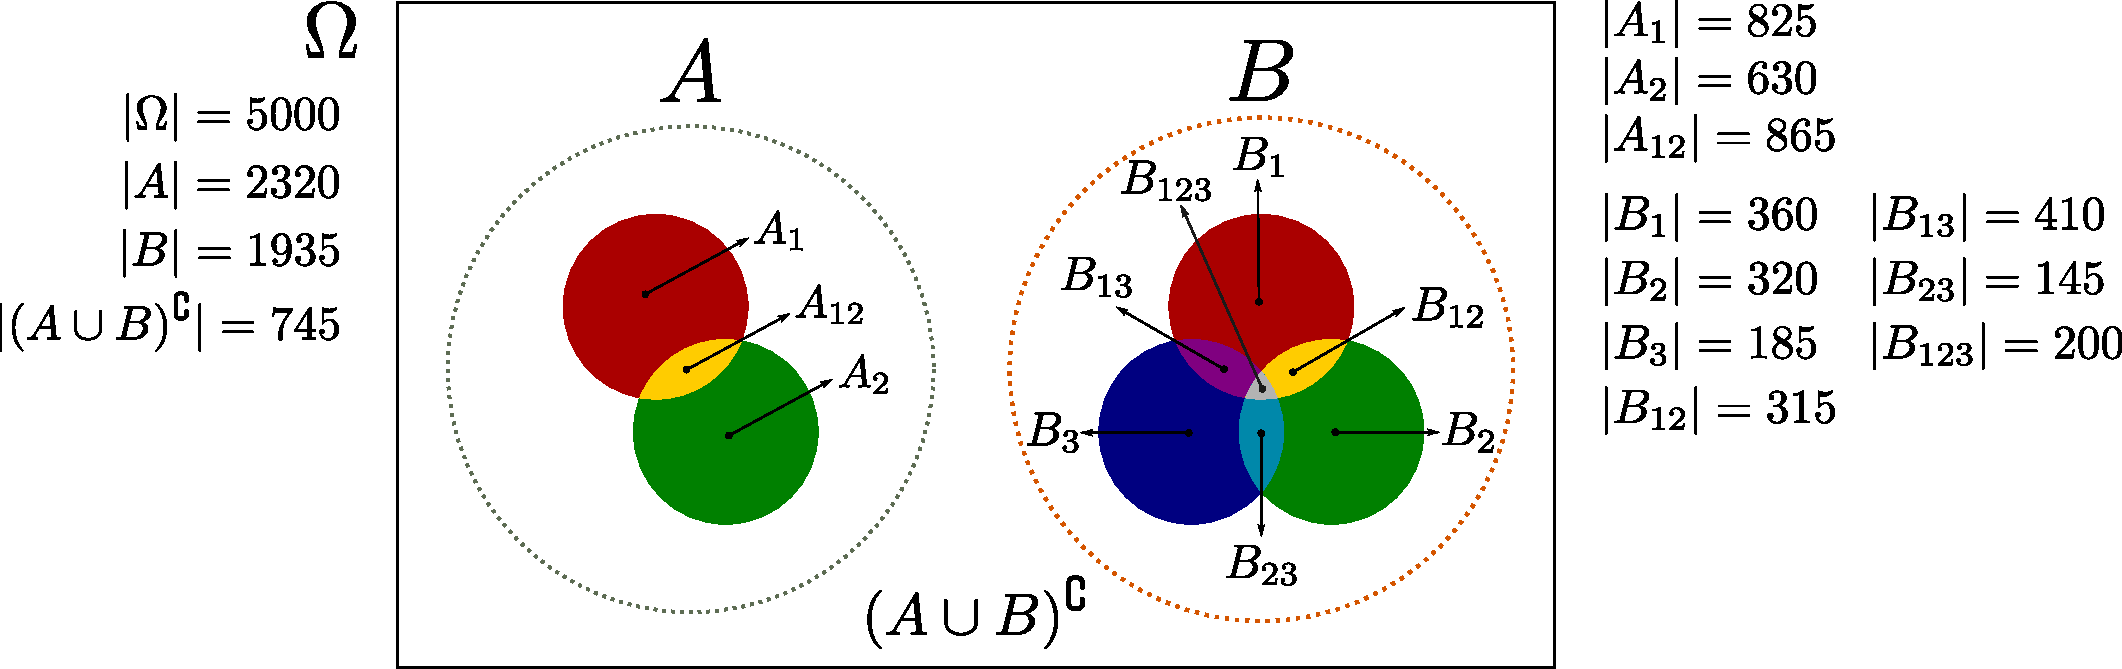
\epsfig{file=./Assets/Venn.pdf,width=1.0\linewidth,clip=}
\caption{Diagrama de Venn que establece relaciones entre los diversos conjuntos previamente definidos}
\label{Fig:F1}
\end{figure}

Como es posible apreciar en el diagrama de Venn presentado en la Figura~\ref{Fig:F1}, el espacio muestral se encuentra conformado a partir de tres subconjuntos principales de este. En primer lugar, los accionistas que se encuentran de acuerdo con la alternativa $A$, corresponden a 2320 individuos. En segundo lugar, es posible establecer el número de accionistas que se encuentran de acuerdo con la alternativa $B$, el cual corresponde a 1935 individuos. Finalmente, el número de individuos que no se encuentran de acuerdo con la alternativa $A$, as\'{i} como la alternativa $B$, corresponde a 745.
\\
\\
Debido a que los accionistas que se encuentran de acuerdo con la alternativa $A$, solo manifestaron su aprobaci\'{o}n con respecto a las alternativas de financiamiento 1 y 2, solo es posible establecer tres subconjuntos de $A$: $A_1$, $A_{12}$ y $A_{2}$, cada uno con una cardinalidad de 825, 865 y 630 individuos, respectivamente.
\\
\\
Por último, con respecto a los accionistas que demostraron una preferencia por la alternativa $B$, es posible conformar seis subconjuntos posibles de elección de opción de financiamiento manifestadas por cada uno de los miembros del conjunto $B$: $B_1$, $B_2$, $B_3$, $B_{12}$, $B_{13}$ y $B_{123}$. Es necesario denotar que la uni\'{o}n de cada uno de los suconjuntos previamente mencionados, corresponde al conjunto global que los contiene. Adem\'{a}s, debido a la inexistencia de accionistas interesados en la alternativa $A$ y $B$ de forma simult\'{a}nea, la intersecci\'{o}n entre estos conjuntos es nula.  
\\

\subsection{Relaci\'{o}n entre la alternativa B y la opci\'{o}n 3}
Se desea establecer si los eventos $B$ y optar por la opci\'{o}n de financiamiento 3 son independientes. Para este fin, es necesario establecer si $\mathrm{P}(3 \vert B) = \mathrm{P}(3)$. Como es posible apreciar en la ecuaci\'{o}n \eqref{eq:e2}, la probabilidad de que ocurra el evento 3 es menor a la probabilidad de que ocurra el evento 3 dado el evento $B$. Esto implica que si este evento ocurriese el espacio de muestreo para el evento 3 es reducido, y por lo tanto, los eventos 3 y $B$ son dependientes.

\begin{alignat}{2}
\mathrm{P}(3 \vert B) &= \mathrm{P}(3) \\
\mathrm{P}(3 \vert B) &= \frac{\vert B_3 \vert + \vert B_{23} \vert + \vert B_{13} \vert + \vert B_{123} \vert}{\vert B \vert} \\
\mathrm{P}(3) &= \frac{\vert B_3 \vert + \vert B_{23} \vert + \vert B_{13} \vert + \vert B_{123} \vert}{\vert \Omega \vert} \\
\mathrm{P}(3) &< \mathrm{P}(3 \vert B) \quad \Rightarrow \quad \mathrm{P}(3 \vert B) \neq \mathrm{P}(3) \qquad \text{\lightning} \label{eq:e2}
\end{alignat}

\subsection{Independencia de los eventos $A$ y $B$}
En primer lugar, debido a que los conjuntos $A$ y $B$ son disyuntos, la probabilidad de $A \cap B$ es equivalente a cero. Adem\'{a}s, debido a que la elecci\'{o}n de una alternativa de exploraci\'{o}n por parte de un accionista es exclusiva, no es posible realizar la elecci\'{o}n de dos alternativa, esto implica que $\mathrm{P}(A \vert B) = 0$. Conforme a la definici\'{o}n de independencia de eventos presentada en (4), se dice que si dos eventos son independientes, entonces, la probabilidad de la intersecci\'{o}n de ambos eventos es distinta de cero. A continuaci\'{o}n se presenta una prueba que establece que los eventos $A$ y $B$ son independientes:

\begin{center}
\begin{twoproof}
\label{step1} $\mathrm{P}(A \cap B) = 0$ & Hip\'{o}tesis \\
\label{step2} $\mathrm{P}(A \vert B) = 0$ & Hip\'{o}tesis \\
\label{step3} $\mathrm{P}(A  \vert B) = \mathrm{P}(A) \Rightarrow \mathrm{P}(A \cap B) \neq 0$  & Definición Independencia \\
\label{step4} $\mathrm{P}(A \vert B) = \mathrm{P}(A) \Rightarrow \text{False}$  & Sustituci\'{o}n (1, 3)\\
\label{step5} $\mathrm{P}(A  \vert B) \neq \mathrm{P}(A)$  & Negaci\'{o}n derecha $\Rightarrow$ (4) \\
\label{step6} $\mathrm{P}(A) = \frac{58}{125}$  &  Aritm\'{e}tica \\ 
\label{step6} $True$ & Sustituci\'{o}n (1,6,5) $\qed$
\end{twoproof}
\end{center}

\subsection{Probabilidad de escoger la alternativa $B$}
\begin{alignat}{4}
\text{P}(B) &= \frac{\vert B \vert}{\vert \Omega \vert} \\
\text{P}(B) &= \frac{1935}{5000} \\
\text{P}(B) &\approx 0.387 \qed
\end{alignat}

\subsection{Probabilidad de escoger la alternativa $B$ y la alternativa $A$}
\begin{alignat}{1}
\text{P}(A \cap B) &= 0 \qed 
\end{alignat}

\subsection{Probabilidad de elegir la opci\'{o}n de financiamiento 1}
\begin{alignat}{4}
\text{P}(1) &= \frac{\vert A_1 \vert + \vert A_{12} \vert + \vert B_1 \vert + \vert B_{12} \vert + \vert B_{13} \vert + \vert B_{123} \vert}{\vert \Omega \vert}  \\
\text{P}(1) &= \frac{119}{200} \\
\text{P}(1) &= 0.595 \qed
\end{alignat}

\subsection{Probabilidad de escoger la alternativa $A$ y las opciones de financiamiento 1 y 2}
\begin{alignat}{4}
\text{P}(A_{12}) &= \frac{\vert A_{12} \vert}{\vert A \vert} \\
\text{P}(A_{12}) &= \frac{865}{2320} \\
\text{P}(A_{12}) &\approx 0.372 \qed
\end{alignat}

\subsection{Probabilidad de elegir exclusivamente la alternativa de financiaci\'{o}n 3}
\begin{alignat}{2}
\text{P}(3) &= \frac{\vert B_{3} \vert}{\vert \Omega \vert} \\
\text{P}(3) &= \frac{39}{1250} \\
\text{P}(3) &= 0.0312 \qed
\end{alignat}

\subsection{Probabilidad de escoger la alternativa $B$ y preferir dos opciones de financiaci\'{o}n}
\begin{alignat}{2}
\text{P}(B_{12} \cup B_{13} \cup B_{23}) &= \frac{\vert B_{12} \vert + \vert B_{13} \vert + \vert B_{23} \vert}{\vert \Omega \vert} \\
\text{P}(B_{12} \cup B_{13} \cup B_{23}) &= \frac{87}{500} \\
\text{P}(B_{12} \cup B_{13} \cup B_{23}) &= 0.174 \qed
\end{alignat}

\subsection{Probabilidad de elegir las opciones de financiaci\'{o}n 1 y 3 exclusivamente, si se conoce que la Alternativa $B$ fue escogida}
\begin{alignat}{2}
\text{P}(B_{13}) &= \frac{\vert B_{13} \vert}{\vert B \vert} \\
\text{P}(B_{13}) &= \frac{82}{387} \\
\text{P}(B_{13}) &= 0.211 \qed
\end{alignat}

\subsection{Probabilidad de escoger la alternativa $A$, si se conoce que la opc\'{o}n de financiaci\'{o}n 1 fue elegida}
\begin{alignat}{2}
\text{P}(A \vert 1) &= \frac{\text{P}(1 \vert A) \text{P}(A)}{\text{P}(1)} \\
\text{P}(A \vert 1) &= \frac{(\text{P}(A_{1} \cup A_{12})\text{P}(A_{1} \cup A_{12} \cup A_2) }{\text{P}(1)} \\
\text{P}(A \vert 1) &\approx 0.247 \qed
\end{alignat}

\section{Cálculo de probabilidades de eventos (Gráficas)}

\begin{figure}
\centering
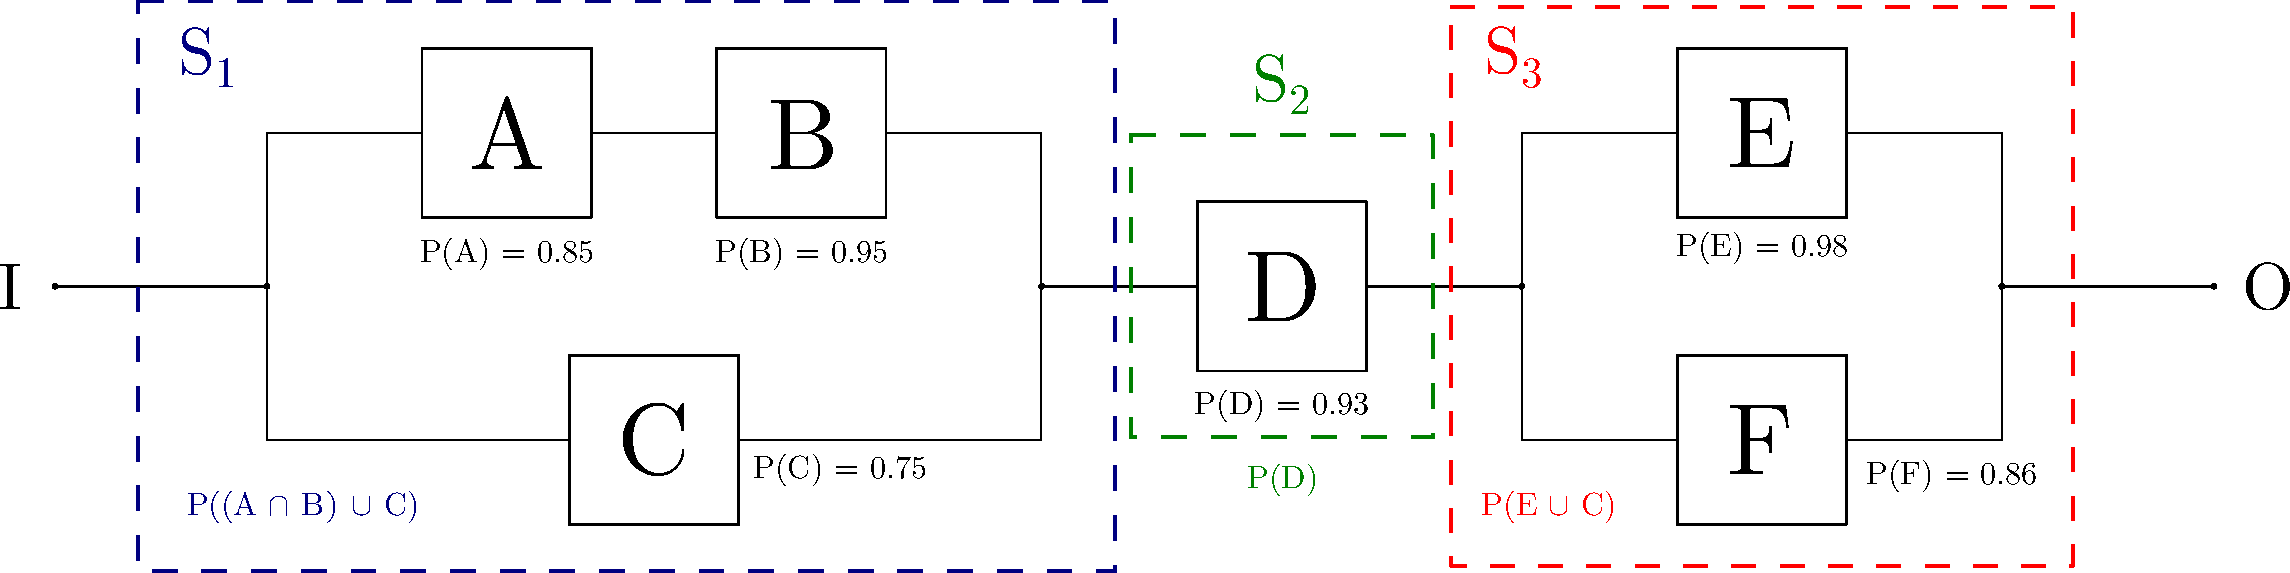
\epsfig{file=./Assets/Circuit.pdf,width=1.0\linewidth,clip=}
\caption{Diagrama l\'{o}gico del circuito que establece relaciones entre los diversos componentes}
\label{Fig:F2}
\end{figure}

Debido a que los eventos son independientes, es posible afirmar que la probabilidad de ocurrencia de la intersecci\'{o}n entre dos eventos, corresponde al producto de las probabilidades de ambos eventos, \textit{i.e.,} $\text{P}(A \cap B) = P(A) \cdot P(B)$. Conforme a esta disposici\'{o}n, a continaci\'{o}n, es posible asignar un valor de probabilidad al evento $W$ \eqref{eq:eq3}, el cual corresponde a la probabilidad de funcionamiento del circuito.

\begin{alignat*}{2}
P(W) &= P(S_1 \cap S_2 \cap S_3) \label{eq:e3} \\
P(W) &= P(S_1)\cdot P(S_2) \cdot P(S_3) \\
P(W) &= P((A \cap B) \cup C) \cdot P(D) \cdot P(E \cup F) \\
P(W) &= (P(A \cap B) + P(C) - P(A \cap B \cap C)) \cdot P(D) \cdot (P(E) + P(F) - P(E \cap F)) \\
P(W) &= (P(A) \cdot P(B) + P(C) - P(A)\cdot P(B) \cdot P(C)) \cdot P(D) \cdot (P(E) + P(F) - P(E \cap F)) \qed \\
P(W) &\approx \boxed{0.882}  
\end{alignat*}

\section{Técnicas de Conteo}
\subsection{Número de resultados posibles en términos de la tabla de posiciones}
$\bullet$ $N$ : Número de posibles resultados en términos de la tabla de posiciones 
\\
\begin{alignat*}{2}
   N &= 8 \text{\textbf{P}} 8 \\
   N &= \frac{8!}{(8-8)!} \\
   N &= 8! \qed  
\end{alignat*}

\subsection{Probabilidad de que dos equipos pertenecientes a la Universidad de los Andes ocupen las dos primeras posiciones}
$\bullet$ $2A$ : 2 Equipos que pertenecen a la Universidad de los Andes ocupan las dos primeras posiciones.
\\
\begin{alignat*}{2}
P(2A) &= \frac{2! \cdot 6!}{8!} \\
P(2A) &= \frac{1}{28} \\
P(2A) &\approx 0.0357 \qed
\end{alignat*}

\subsection{Probabilidad de que los equipos de Comunicación, Derecho y Administración ocupen las tres primeras posiciones (Sin importar el orden)}
$\bullet$ $CDA$ : Los equipos de Comunicación, Derecho y Administración ocupen las tres primeras posiciones. 
\\
\begin{alignat*}{2}
P(CDA) &= \frac{3! \cdot 5!}{8!} \\
P(CDA) &= \frac{1}{56} \\
P(CDA) &\approx 0.0178 \qed
\end{alignat*}

\subsection{Probabilidad de que las tres primeras posiciones sean ocupadas por los equipos de Ingeniería, Matemáticas y Diseño (Respectivamente)}
$\bullet$ $IMD$ : Los equipos de Ingeniería, Matemáticas y Diseño ocupan las tres posiciones de la tabla de posiciones (En orden).
\\
\begin{alignat*}{2}
P(IMD) &= \frac{2! \cdot 5!}{8!} \\
P(IMD) &= \frac{1}{168} \\
P(IMD) &\approx \num{5.95e-3} \qed
\end{alignat*}

\subsection{Número de formas posibles de ordenar ocho equipos en dos grupos que contienen cuatro elementos cada uno}
$\bullet$ $C$ :  Número de formas posibles de ordenar ocho equipos en dos grupos que contienen cuatro elementos cada uno
\\
\begin{alignat*}{2}
C &= \binom{8}{4} \\
C &= \frac{8!}{4! \cdot 4!} \\
C &= 70 \qed
\end{alignat*}

\subsection{Probabilidad de que en un mismo grupo quede únicamente un equipo de Ingeniería y el equipo de Diseño}
$\bullet$ $ID$ : En un mismo grupo queda únicamente un equipo de Ingeniería y el equipo de Diseño.
\\
\begin{alignat*}{2}
P(ID) &= \frac{\binom{2}{1} \binom{1}{1} \binom{5}{2} \binom{3}{3}}{\binom{8}{4}} \\
P(ID) &= \frac{2}{7} \\
P(ID) &\approx 0.285 \qed 
\end{alignat*}

\subsection{Probabilidad de que los equipos de las facultades de Ingeniería queden de primeros en cada grupo}
$\bullet$ $I$ : La final del torneo se disputa entre dos equipos de Ingeniería. \\
$\bullet$ $I_1$ : El ganador del equipo 1, es un equipo de Ingeniería. \\
$\bullet$ $I_2$ : El ganador del equipo 2, es un equipo de Ingeniería.
\\
\begin{alignat*}{2}
P(I) &= P(I_1)\cdot P(I_2) \\
P(I_1) &= \frac{3!}{4!} \\
P(I_1) &= \frac{1}{4} \\
P(I_2) &= P(I_1) \\
\Rightarrow P(I) &= \frac{1}{16}
\end{alignat*}

\section{Teorema de Bayes y Árboles de Probabilidad}
\subsection{Árbol de probabilidad}
Ver Figura~\ref{Fig:F3}

\tikzstyle{level 1}=[level distance=2.5cm, sibling distance=7cm]
\tikzstyle{level 2}=[level distance=3.5cm, sibling distance=3.5cm]
\tikzstyle{level 3}=[level distance=3.5cm, sibling distance=2.5cm]

% Define styles for bags and leafs
\tikzstyle{bag} = [text width=4em, text centered]
\tikzstyle{end} = [circle, minimum width=3pt,fill, inner sep=0pt]
\begin{figure}[t]
\centering
\begin{tikzpicture}[grow=right, sloped]
\node[end] {}
    child {
        node[end] {}        
            child {
                node[end, label=right:
                    {$P(N^{\complement})= 0.5 \cdot 0.35$}] {}
                edge from parent
                node[above] {$P(N_2^{\complement} \vert N_1^{\complement})$}
                node[below]  {$0.5$}
            }
            child {
                %node[end, label=right:
                    %{$P(W_1\cap B_2)=\frac{4}{7}\cdot\frac{5}{9}$}] {}
                    node[end]{}
                child
                {
                     node[end, label=right:
                     {$P(N^{\complement})=0.5\cdot 0.5 \cdot 0.35$ }] {}
                    %node[end, label=right: {$P(N^{\complement}) = 0.5 \cdot 0.3 \cdot 0.65$}]{}
                    edge from parent
                       node[above] {$P(N_3^{\complement})$}
                       node[below] {$0.5$}
                }
                child
                {
                     node[end, label=right:
                     {$P(N)=0.5\cdot 0.5 \cdot 0.35$ }] {}
                    %node[end, label=right: {$P(N) = 0.5 \cdot 0.3 \cdot 0.65$}]{}
                    edge from parent
                       node[above] {$P(N_3)$}
                       node[below] {$0.5$}
                }
                edge from parent
                node[above] {$P(N_2 \vert N_1^{\complement})$}
                node[below]  {$0.5$}
            }
            edge from parent 
            node[above] {$P(N_1^{\complement})$}
            node[below]  {$0.35$}
    }
    child {
        node[end] {}        
        child {
%                node[end, label=right:
%                    {$P(B_1\cap W_2)=\frac{3}{7}\cdot\frac{3}{9}$}] {}
                node[end]{}
                child
                {
                     node[end, label=right:
                     {$P(N^{\complement})=0.5\cdot 0.3 \cdot 0.65$ }] {}
                    %node[end, label=right: {$P(N^{\complement}) = 0.5 \cdot 0.3 \cdot 0.65$}]{}
                    edge from parent
                       node[above] {$P(N_3^{\complement})$}
                       node[below] {$0.5$}
                }
                child
                {
                     node[end, label=right:
                     {$P(N)=0.5\cdot 0.3 \cdot 0.65$ }] {}
                    %node[end, label=right: {$P(N) = 0.5 \cdot 0.3 \cdot 0.65$}]{}
                    edge from parent
                       node[above] {$P(N_3)$}
                       node[below] {$0.5$}
                }                
                edge from parent
                node[above] {$P(N_2^{\complement} \vert N_1)$}
                node[below]  {$0.3$}
            }
            child {
                node[end, label=right:
                    {$P(N) = 0.65\cdot0.7$}] {}
                edge from parent
                node[above] {$P(N_2 \vert N_1)$}
                node[below]  {$0.7$}
            }
        edge from parent         
            node[above] {$P(N_1)$}
            node[below]  {$0.65$}
    };
\end{tikzpicture}
\caption{Árbol de probabilidades que describe y modela la situación presentada}
\label{Fig:F3}
\end{figure}

\subsection{Probabilidad de que Nairo Quintana/Chris Froome gane la Vuelta a España}
\begin{alignat*}{2}
P(N) &= P(N_1) \cdot (P(N_2 \vert N_1) + P(N_2^{\complement} \vert N_1) \cdot P(N_3)) + P(N_1^{\complement}) \cdot P(N_2 \vert N_1^{\complement}) \cdot P(N_3) \\ 
P(N) &= \frac{16}{25} \\
P(N) &= 0.64 \qed \\ \\
\Rightarrow P(N^{\complement}) &= 1 - P(N) \\
            P(N^{\complement}) &= 0.36 \qed
\end{alignat*}

\subsection{Probabilidad de ganar la Vuelta España tras ganar dos validas consecutivas}
$\bullet$ $2G$ : Probabilidad de ganar la Vuelta España tras ganar dos validas consecutivas 
\\
\begin{alignat*}{2}
P(2G) &= P(N_1) \cdot P(N_2 \vert N_1) + P(N_1^{\complement}) \cdot P(N_2^{\complement} \vert N_1^{\complement}) \\
P(2G) &= 0.63 \qed
\end{alignat*}

\subsection{Probabilidad de que Chris Froome gane la etapa número 11, dado que ganó la etapa 16}
\begin{alignat*}{2}
P(N_1^{\complement} \vert N_2^{\complement}) &= \frac{P(N_2^{\complement} \vert N_1^{\complement})\cdot P(N_1^{\complement})}{P(N_2^{\complement})} \\ 
\\
P(N_2^{\complement}) &= P(N_1)\cdot P(N_2^{\complement} \vert N_1) + P(N_1^{\complement}) \cdot P(N_2^{\complement} \vert N_1^{\complement}) \\
P(N_2^{\complement}) &= 0.37 \\
\\
\Rightarrow P(N_1^{\complement} \vert N_2^{\complement}) &= 0.283 \qed
\end{alignat*}

\section{Variables Aleatorias Discretas}
\begin{figure}[!htbp]
\centering
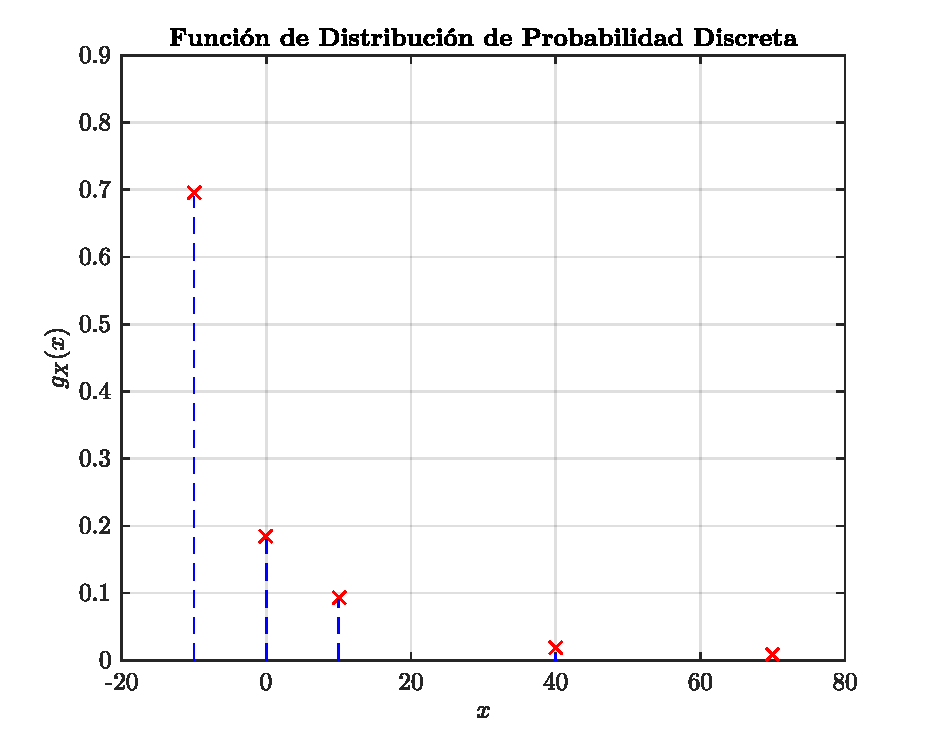
\epsfig{file=./Assets/discrete.pdf,width=0.7\linewidth,clip=}
\caption{Gráfica de la función de probabilidad discreta, $g_X(x)$}
\label{Fig:F4}
\end{figure}
\subsection{Función de probabilidad discreta}
\begin{alignat*}{2}
\mathbb{R}(x) &= \{-10, 0, 10, 40, 70\} \\\\
 g_{X}(x) &= P(x) =
   \begin{dcases}
     \sfrac{25}{36} & x = -10 \\
     \sfrac{5}{27} & x = 0 \\
     \sfrac{5}{54} & x = 10 \\
     \sfrac{1}{54} & x = 40 \\
     \sfrac{1}{108} & x = 70 \\
     0 & \text{d.l.c}
   \end{dcases} \\
   &\boxed{\sum_{x \in \mathbb{R}(x)} g_X(x) = 1} \qed
\end{alignat*}

\subsubsection{Gráfica $g_X(x)$}
Ver Figura~\ref{Fig:F4}.

\subsection{Función de probabilidad acumulada}
\begin{equation*}
G_{X}(x) = P(x \leq X) = 
\begin{dcases}
     0 & -10 < x \\
     \sfrac{25}{36} & -10 \leq x < 0 \\
     \sfrac{95}{108} & 0 \leq x < 10 \\
     \sfrac{35}{36} & 10 \leq x < 40  \\
     \sfrac{107}{108} & 40 \leq x < 70 \\
     1 & x \geq 70 
   \end{dcases}
\end{equation*}
\begin{figure}[!htbp]
\centering
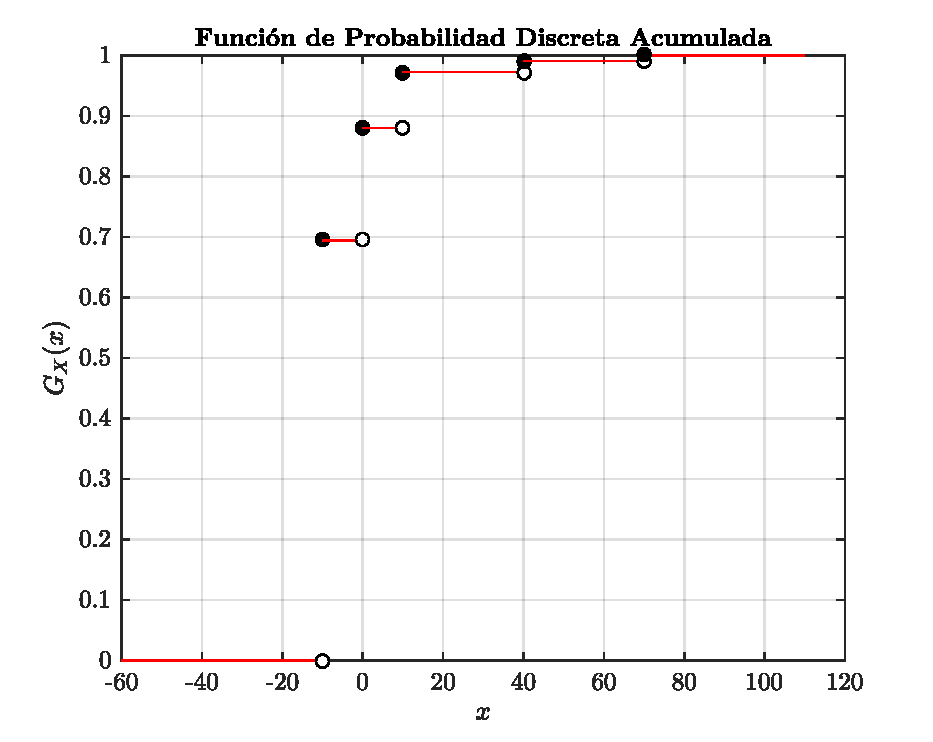
\epsfig{file=./Assets/cdf.pdf,width=0.7\linewidth,clip=}
\caption{Gráfica de la función de probabilidad acumulada discreta, $G_X(x)$}
\label{Fig:F5}
\end{figure}

\subsubsection{Gráfica $G_X(x)$}
Ver Figura~\ref{Fig:F5}.

\subsection{Valor esperado y desviaci\'{o}n est\'{a}ndar}
\subsubsection{Valor esperado}
\begin{alignat}{2}
\mathbb{E}[x] &= \sum_{x \in \mathbb{R}(x)} x_i \cdot g_X(x) \\
\mathbb{E}[x] &= -\frac{125}{27} \\
\mathbb{E}[x] &\approx -4.6629 \label{eq:e4}
\end{alignat}
\subsubsection{Desviaci\'{o}n est\'{a}ndar}
\begin{alignat}{2}
\text{Var}[x] &= \mathbb{E}[x^2] - (\mathbb{E}[x])^2 \\ \\
\mathbb{E}[x^2] &= \sum_{x \in \mathbb{R}(x)} x_i^2 \cdot g_X(x) \\
\mathbb{E}[x^2] &= \frac{4150}{27} \\
(\mathbb{E}[x])^2 &= \frac{15625}{729} \\ \\
\Rightarrow \text{Var}[x] &\approx 132.27 \\
\sigma &= \sqrt{\text{Var}[x]} \\
\sigma &\approx 11.50 \label{eq:e5}
\end{alignat}

Conforme al valor esperado obtenido en \eqref{eq:e4}, es posible afirmar que un jugador en promedio tiende a perder cuatro dólares por cada ronda jugada. Esto implica que el juego resulta comportarse de forma lucrativa para el ente/persona que se encuentre encargada de recaudar el dinero apostado por parte de los jugadores, y en general, reduce la probabilidad de que el jugador pueda obtener alguna ganancia al apostar.
\\
\\
Adem\'{a}s, es necesario denotar que la probabilidad de obtener una ganancia neta mayor a 0, es casi cercana a cero, en la medida que la media y los valores centrales se encuentran concentrados en torno a valores de ganancia negativos. Es posible evidenciar este comportamiento de la función al considerar la desviaci\'{o}n est\'{a}ndar \eqref{eq:e5} ($\sigma$) como una medida de dispersi\'{o}n de la informaci\'{o}n de la funci\'{o}n con respecto a la media; en el presente caso, debido a que el valor de la desviaci\'{o}n est\'{a}ndar posee una magnitud alta, es posible afirmar que los valores se encuentran alejados de la media.


\subsection{Acerca de generar lucro por parte de los jugadores}
Debido a que el valor esperado se encuentra en la región de pérdidas de dinero netas, todo jugador que apueste durante una partida del presente juego, tiene una mayor probabilidad de perder dinero, y por lo tanto, la probabilidad de obtener lucro y ganancia resulta ser reducida.

\section{Variables Aleatorias Continuas}
\subsection{Definci\'{o}n Funci\'{o}n de densidad de Probabilidad}
\begin{equation*}
f_{X}(x) =  
\begin{dcases}
   x^2 & 0 \leq x < 1 \\
   k  & 1 \leq x < \sfrac{4}{3} \\
   -\sfrac{3x}{2} + 3 &  \sfrac{4}{3} \leq x \leq 2 \\
   0 & \text{d.l.c}
\end{dcases}
\end{equation*}

\begin{alignat}{2}
\int_{\mathbb{R}(x)} f_{X}(x) = 1
\end{alignat}
\begin{alignat*}{2}
\int_{x = 0}^{1} x^2 ~\text{d}x  + \int_{x = 1}^{\sfrac{4}{3}} k ~\text{d}x + \int_{x = \sfrac{4}{3}}^{2} (-\frac{3}{2}x + 3) ~\text{d}x &= 1 \\
\left.(\frac{x^3}{3})\right|_{x = 0}^1 + \bigg(kx\bigg)\bigg|_{x = 1}^{\sfrac{4}{3}} + \left.(-\frac{3x^2}{4} + 3x)\right|_{x = \sfrac{4}{3}}^2  &= 1 \\
\end{alignat*}
\begin{equation*}
k = 1 \qed
\end{equation*}
\begin{equation*}
f_{X}(x) =  
\begin{dcases}
   x^2 & 0 \leq x < 1 \\
   1  & 1 \leq x < \sfrac{4}{3} \\
   -\sfrac{3x}{2} + 3 &  \sfrac{4}{3} \leq x \leq 2 \\
   0 & \text{d.l.c}
\end{dcases}
\end{equation*}

\begin{figure}[!htbp]
\centering
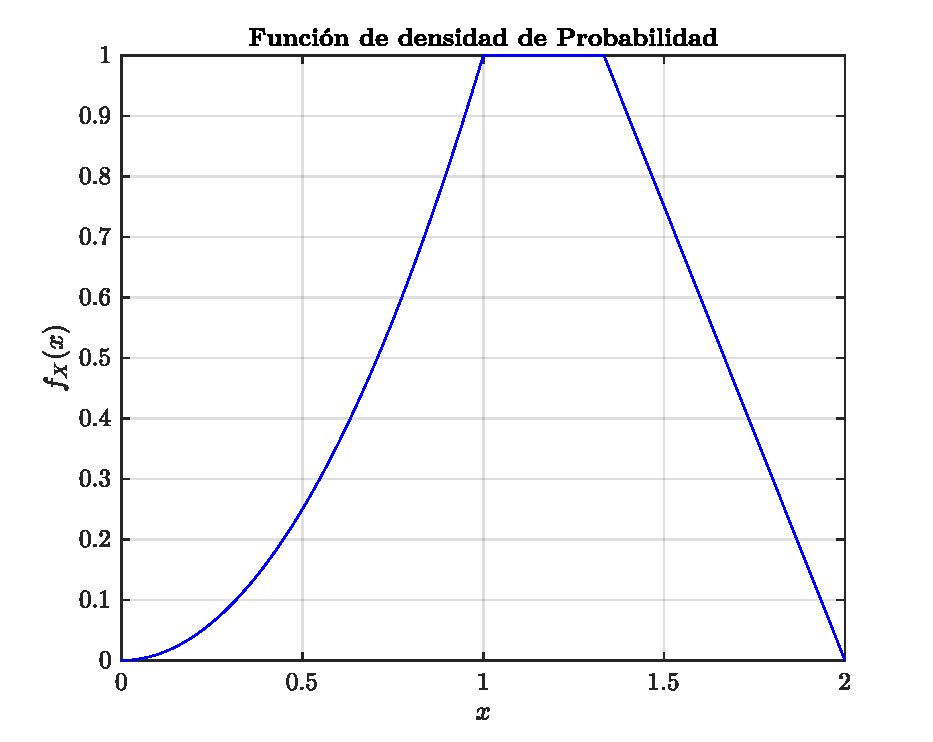
\epsfig{file=./Assets/pdf.pdf,width=0.7\linewidth,clip=}
\caption{Gráfica de la función de densidad de probabilidad, $f_X(x)$}
\label{Fig:F6}
\end{figure}



\subsection{Funci\'{o}n distribuci\'{o}n acumulada}
\begin{equation*}
f_{X}(x) =  
\begin{dcases}
   0   & x \leq 0 \\
   \sfrac{x^3}{3} & 0 \leq x < 1 \\
   x - \sfrac{2}{3}  & 1 \leq x < \sfrac{4}{3} \\
   -\sfrac{3x^2}{4} + 3x - 2 &  \sfrac{4}{3} \leq x \leq 2 \\
   1 & x \geq 2
\end{dcases}
\end{equation*}

\begin{figure}[!htbp]
\centering
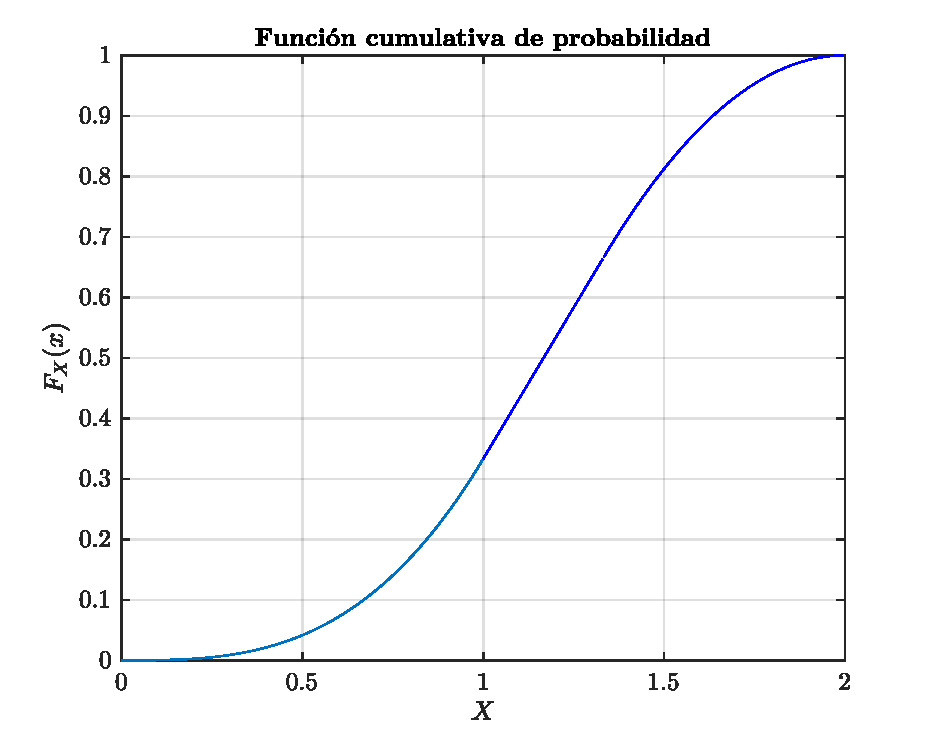
\epsfig{file=./Assets/cpf.pdf,width=0.7\linewidth,clip=}
\caption{Gráfica de la función cumulativa de probabilidad, $F_X(x)$}
\label{Fig:F6}
\end{figure}


\subsection{Valor esperado y Desviaci\'{o}n est\'{a}ndar}
\begin{alignat*}{2}
\mathbb{E}[x] = \int_{x = 0}^{1} x^2 \cdot x ~\text{d}x + \int_{x = 1}^{\sfrac{4}{3}} 1 \cdot x ~\text{d}x  + \int_{x = \sfrac{4}{3}}^{2} (-\frac{3x}{2} + 3) \cdot x ~\text{d}x
\end{alignat*}
\begin{alignat*}{2}
\mathbb{E}[x] = \frac{113}{108} \qed
\end{alignat*}
\begin{alignat*}{2}
\text{Var}[x] = \mathbb{E}[x^2] - (\mathbb{E}[x])^2 \\ 
\end{alignat*}
\begin{alignat*}{2}
\mathbb{E}[x^2] = \int_{x = 0}^{1} x^2 \cdot x^2 ~\text{d}x + \int_{x = 1}^{\sfrac{4}{3}} 1 \cdot x^2 ~\text{d}x  + \int_{x = \sfrac{4}{3}}^{2} (-\frac{3x}{2} + 3) \cdot x^2 ~\text{d}x
\end{alignat*}
\begin{alignat*}{2}
\mathbb{E}[x^2] &= \frac{596}{405} \qed \\ \\
\text{Var}[x] &\approx 0.376 \\
\sigma &\approx 0.61 \qed
\end{alignat*}

\subsection{Probabilidad de ser atendido en exactamente una hora}
\begin{alignat*}{2}
P(x = 1) = 0 \qed
\end{alignat*}

\subsection{Probabilidad de ser atendido entre 1.25 y 1.75 horas}
\begin{alignat*}{2}
P(1.25 \leq x \leq 17.5) &= F_X(1.75)-F_X(1.25) \\
P(1.25 \leq x \leq 17.5) &\approx 0.369
\end{alignat*}

\subsection{Probabilidad de esperar entre entre 1.25 y 1.75 horas, dado que m\'{a}s de una hora ya transcurri\'{o}}
\begin{alignat*}{2}
P(1.25 \leq x \leq 17.5 \vert x > 1) &= \frac{P(1.25 \leq x \leq 17.5 \cap x > 1)}{P(x > 1)} \\
P(1.25 \leq x \leq 17.5 \vert x > 1) &= \frac{P(1.25 \leq x \leq 17.5) \cdot P(x > 1)}{1 - P(x \leq 1)} \\
P(1.25 \leq x \leq 17.5 \vert x > 1) &= P(1.25 \leq x \leq 17.5) \\
P(1.25 \leq x \leq 17.5 \vert x > 1) &= 0.369 \qed
\end{alignat*}

\begin{figure}[!htbp]
\centering
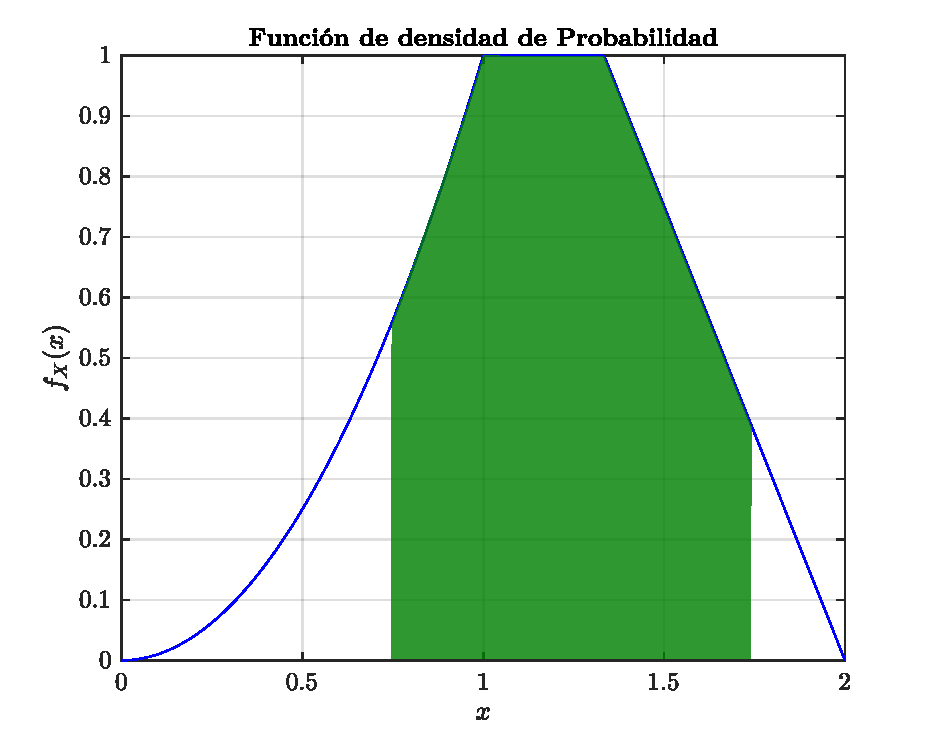
\epsfig{file=./Assets/pdf_2.pdf,width=0.7\linewidth,clip=}
\caption{Descripci\'{o}n gr\'{a}fica del intervalo descrito previamente}
\label{Fig:F7}
\end{figure}


% ------------------------------------------------------------------------------
% End document
% ------------------------------------------------------------------------------
\end{document}
